\chapter{Interacting QFT}
\section{Introduction and examples}
Theories discussed so far are Klein-Gordon theory (spin $0$) $$\lag_{KG} = \frac{1}{2}\partial_\mu\phi\partial^\mu\phi - \frac{m^2}{2}\phi^2$$ and Dirac theory (spin $\frac{1}{2}$) $$\lag_D = \bar{\psi}(i\slashed{\partial} - m) \psi $$

There is also $\lag_{EM} = -\frac{1}{4}F_{\mu\nu}F^{\mu\nu}$ with $F_{\mu\nu} = \partial_\mu A_\nu - \partial_\nu A_\mu$ for a massless vector filed. Its quantiasation gives photon

One thing they have in common is quadratic in the fields. As result:
\begin{itemize}
	\item linear field equations
	\item exact quantisation
	\item multi-particle states without scattering or interaction
	\item linear fourier decompositions , no mementum changes
\end{itemize}

To have an interacting theory with scattering, need higher powers in the field in the Lagrangians. A few examples are following
\paragraph{scalar $\phi^4$ theory}
\begin{align}
	\lag = \lag_{KG} + \frac{\lambda}{4!} \phi^4
\end{align}
need positive sign $\lambda > 0$ for a stable theory, otherwise classical energy can be arbitarily negative.

Equation of motions
\begin{align}
	(\partial^2+ m ^2) \phi = -\frac{\lambda}{3!} \phi^3
\end{align}
is nonlinear, cannot be solved by Fourier decomposition.

\paragraph{Yukawa-theory}
\begin{align}
	\lag = \lag_{KG} + \lag_{D} - g \bar{\psi}\psi \phi
\end{align}
It is originally developed as a theory for nuclear forces with $\psi$ nucleon, $\phi$ pion. In the Standard Model it is similar to interactions in Higgs mechanism.
\paragraph{Quantum Electrodynamics (QED)}
\begin{align}
	\lag = \lag_{EM} + \lag_{D} - eA_\mu \bar{\psi} \gamma^\mu \psi
\end{align}
descreibes electrons, their antiparticles positrons and photons.

\paragraph{Yang-Mills theory}
generalises $\lag_{EM}$ with terms like $A^4$ or $A^2 \partial A$
\paragraph{Scalar QED}
descreibes pions and photons
\begin{align}
	\begin{split}
		\lag &= \lag_{EM} + D_\mu \phi D^\mu\phi^* - m^2 |\phi|^2 \\
			 &= \lag_{EM} + \partial_\mu\phi\partial^\mu\phi^* - m^2 \phi\phi^* + ie A_\mu(\phi\partial^\mu\phi^* - \phi^* \partial^\mu\phi) + e^2 A_\mu A^\mu \phi\phi^*
	\end{split}
\end{align}
\paragraph{Remarks}
\begin{enumerate}
	\item Interaction terms in $H_\text{int} = \int \dd^3 \ham_\text{int} = - \int\dd^3x\lag_\text{int}$ always involves products of fields at the same point $\pmb{x}$. It ensures causality, no "instant at a distance".
	\item There are no derivative interactions. These may complicate quantisation as $$\pi(\pmb{x}) = \frac{\partial\lag}{\partial(\partial_0 \phi(\pmb{x}))}$$
	\item Why the examples above? There must be zillions of theories (Lagrangians)? \\
			We have the criterion of \textbf{renormalizability}. Note the mass dimensions of fields;
			\begin{align*}
				[S] = 1 \, \text{so} \, [\lag] = [M]^4 \, \Rightarrow [\phi] = [M] ,\, [\psi] = [M]^{\frac{3}{2}} ,\, [A_\mu] = [M]
			\end{align*}
			So in all the interaction terms indicated above, the coupling constant $\lambda$, e, g are all \textbf{dimensionless}!\\
			Can add $-\frac{\mu}{3!}\phi^3$ to the $\phi^4$ theory. This leads to $[\mu] = [M]$ and all these generate renormalisable interactions. \\
			All higher interaction terms require coupling constants of \textbf{negative} mass dimension. e.g. $G\bar{\psi}\psi\bar{\psi}\psi$ and then $[G] = [M]^{-2}$. These are nonrenormalisable and create trouble when performing higher-order calculation in perturbation theory.
			(with energy cutoff; corrections $~G\Lambda^2$, $\Lambda \rightarrow \infty$)
		\item we haven't quantised the photon yet. The reason is that its is a vector field, i.e. 4 degrees of freedom, but photon has just $2$ physical polarisaion states. It is linked to gauge symmetry and complicates quantisation somewhat.
\end{enumerate}
\section{The interaction picture}
Consider the $\phi^4$ theory, 
\begin{align}
\lag_{int} = -\frac{\lambda}{4!} \phi(x)^4
\end{align}
Hamiltonian $H = H_0 + H_{int}$ with 
\begin{align}
	H_0 &= \int\dd^3 x \left\{ \frac{1}{2}\pi^2(x) + \frac{1}{2}(\pmb{\nabla}\phi)^2 + \frac{1}{2}m^2\phi^2 \right\}\\
	H_{int} &= -\int\dd^3x \lag_{int} = \frac{\lambda}{4!}\int\dd^3x \phi^4 
\end{align}

Interaction picture means that operators evolve in time using $H_0$ (only), in particular 
\begin{align}
	\phi_I(t,\pmb{x}) = e^{iH_0t}\phi(\pmb{x})e^{-iH_0t}
\end{align}

Time-dependence of the free field, obeys classical equation of motion $\left(\partial^2+m^2 \right)\phi_I(t,\pmb{x}) = 0$. Solution in terms if fourier modes as before:
\begin{align}
	\phi_I = \int \frac{\dd^3 p}{(2\pi)^3\sqrt{2E_p}} (a^I_{\pmb{p}}e^{-ipx} + a^{I\,\dagger}_{\pmb{p}}e^{+ipx})
\end{align}
as in the free theory with standard commutation relations $[a^I_{\pmb{p}}, a^{I\,\dagger}_{\pmb{p}}] = (2\pi)^3\delta^{(3)}(\pmb{p}-\pmb{p}')$. The state satisfing $a^I_p \ket{0} = 0$ is the vacuum of the free, noninteratcting theory.

Relation between interaction and Schrödinger picure states:
\begin{align}
	\ket{\phi_I(t)} = e^{iH_0t}{\ket{\psi_S(t)}}
\end{align}
Schrödinger equation becomes: 
\begin{align}
	i\frac{\partial}{\partial t}\ket{\psi_S} &= (H_0 + H_\text{int})\ket{\psi_S} \notag\\
	\text{LHS} &= i \frac{\partial}{\partial t} ( e^{-iH_0t}\ket{\phi_I}) = H_0 e^{-iH_0t}\ket{\phi_I} + e^{-iH_0t}i\frac{\partial}{\partial t}\ket{\phi_I} \notag\\
	\text{RHS}														&= \left(H_0 + H_\text{int}\right)e^{-iH_0t}\ket{\phi_I} \notag\\
	\Rightarrow i\frac{\partial}{\partial t}\ket{\phi_I} &= e^{iH_0t}H_{int} e^{-iH_0t} = H_I(t)\ket{\phi_I} \label{math:int-schr}
\end{align}
with $H_I$ interaction Hamiltonian in the interaction picture. Clearly
\begin{align}
	H_I = \frac{\lambda}{4!}\int\dd^3x\phi_I^4(x) \notag
\end{align}

What is the solution of \ref{math:int-schr} for the time evolution of $\ket{\phi_I(t)}$? Define time-evolution operator in the interaction picture.
\begin{align}
	\ket{\phi_I(t)} &= U(t,t_0)\ket{\phi_I(t_0)}\label{math:int-schr2}\\
	\text{where} \; U(t,t_0) &= e^{iH_0(t-t_0)}e^{-iH(t-t_0)} 
\end{align}

With \ref{math:int-schr} and \ref{math:int-schr2}:
\begin{align}
	i\frac{\partial}{\partial t} U(t,t_0) = H_I(t)U(t,t_0)
\end{align}

To solve with boundary conditions: $U(t_0, t_0) = \id$. The formal solution:
\begin{align}
	U(t,t_0) = 1 - i \int_{t_0}^t \dd t' H_I(t')U(t',t_0) \notag
\end{align}

Substitute back in and we get:
\begin{align}
	U(t,t_0) = 1- i \int_{t_0}^t \dd t' H_I(t') + (-i)^2 \int_{t_0}^t \dd t' \int^{t'}_{t_0} \dd t'' H_I(t') H_I(t'') + \dots
\end{align}

Ranges of integration: $H_I$ in the product is automatically time-ordered.

\begin{figure}[ht]
	\centering
	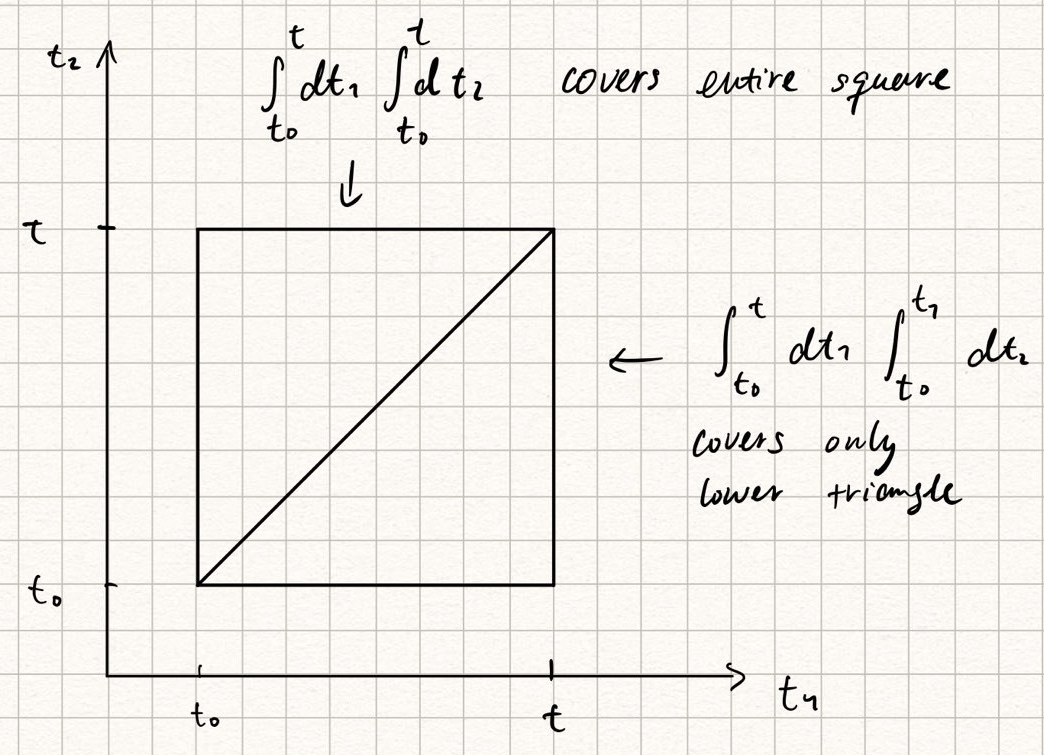
\includegraphics[width=0.65\linewidth]{4-2-triangle.jpg}
	\caption{Time ordering}
	\label{fig:4-2-triangle}
\end{figure}

Upper triangle has the wrong time order. We are going to "repair" it by hand.
\begin{align}
	U(t,t_0) &= 1-i\int_{t_0}^t \dd t' H_I(t') + \frac{(-i)^2}{2} \int_{t_0}^t \dd t' \int^{t'}_{t_0} \dd t'' T(H_I(t') H_I(t'')) + \dots \notag\\
			 &= \sum_{n=0}^{\infty} \frac{(-i)^n}{n!}\int_{t_0}^t \dd t_1 \dots \int_{t_0}^t \dd t_n T(H_I(t_1) \dots H_I(t_n))  \notag\\
			 &= T \exp{-i\int_{t_0}^t \dd t' H_I(t') }
\end{align}

It is interesing for scattering to transition into asymptotic state for $t \rightarrow \infty$
\begin{align}
	S = \lim_{t \rightarrow \infty} U(t,-t) &= T \exp{-i \int_{-\infty}^\infty \dd t H_I(t)} \\
	 &\stackrel{\phi^4}{=} T \exp{-i\int \dd^4 x \frac{\lambda}{4!} \phi_I^4(x)} \notag
\end{align}
Both $U$ and $S$ are formally unitary

Composition law for time evolution operator: 
\begin{align}
	U(t_2, t_0) = U(t_2, t_1) U(t,t_0) = U(t_2, t_1) U(t_0, t_1)^\dagger
\end{align}

\subsection{Scattering amplitudes and the S-matrix}
Take $\ket{i}$ the initial (multi-particle) state and $\ket{f}$ the final (multi-particle) state. Time evolution of $\ket{i}$ then is
$$\lim(t\rightarrow\infty)U(t,-\infty) \ket{i} = S \ket{i}$$

Probability that $\ket{i}$ evolves into $\ket{f}$ is proporional to the squared "\textbf{S-matrix element}"
\begin{align}
	\left|	\braket{f,\, t\to \infty | i, t\rightarrow - \infty}\right|^2 = \left| \braket{f|S|i} \right|^2 = \left| S_{fi} \right|^2
\end{align}

The nontrivial part of the S-matrix is the T-matrix:
\begin{align}
	S_{fi} \defeq \delta_{fi} + iT_{fi}
\end{align}

Use momentum conservation (from translation invariance) to define matrix element
\begin{align}
	S_{fi} = \delta_{fi} + i(2\pi)^4 \delta^{(4)}(p_f - p_i) M_{fi}
\end{align}
$M_{fi}$ measures "genuine scattering" from $\ket{i}$ to $\ket{f}$.

How are we going to calculate correlation functions in the interacting theory:
\begin{align}
	\braket{\Omega |  \ T \phi(x)\phi(y) | \Omega}	
\end{align}
or more generally $\braket{\Omega | T \phi(x_1)\phi(x_2)\dots | \Omega}$, where $\ket{\Omega}$ is the vaccum/ground state of the interacting theory and $\phi(x)$ the Heisenberg operators.

Ignore $\ket{\Omega} \neq \ket{0}$ for the moment other than saying: we want to study the time evolution from the vacuum at $t\rightarrow - \infty$ to $t \rightarrow + \infty$. So rewriting in terms $\phi_I(x)$, assuming $x^0 > y^0$ for now:
\begin{align}
	\braket{0 | U(\infty, x^0) \phi_I(x^0)  U(x^0, y^0) \phi_I(y^0)U(y^0, -\infty) | 0}  = \braket{0|T(\phi_I(x)\phi_I(y)S)|0}
\end{align}
still holds if $x^0 < y^0$ because of $T$.

Now $\ket{\Omega} \neq \ket{0}$: this can be taken care of by dividing out the time evolution of the (free) vacuum $\braket{0|S|0}$, so
\begin{align}
	\braket{\Omega | T(\phi(x)\phi(y))|\Omega} \notag\\
	&= \frac{\braket{0 | T(\phi_I(x)\phi_I(y)S)|0}}{\braket{0|S|0}} \\
	&\stackrel{\phi^4}{=} \frac{
		\braket{0 | T {\phi_I(x)\phi_I(y)\exp{-i\int\dd^4x' \frac{\lambda}{4!}\phi^4(x')}}| 0}
		}{
		\braket{0 | T {\exp{-i\int\dd^4x' \frac{\lambda}{4!}\phi^4(x')}}| 0}
}\notag
\end{align}
Proof can be found in Peskin. It will also be illustrated parctically later ("vacuum bubbles").

Perturbation theory is viable when $\lambda$ (or some other coupling) is "small" and then expands $U(t,t_0)$ or $S$ in powers of $\lambda$.

\section{Wick's theorem}
From now on drop the subscript for interaction pictire fields $\phi_I(x) \rightarrow \phi(x)$.

Want to calculate stuff like $\braket{0 | T\phi(x_1)\dots\phi(x_n)S | 0}$ in pert. theory; so e.g. at order $\lambda^n$. So 
\begin{align}
\frac{1}{n!} \left( -i\frac{\lambda}{4!} \right)^n \int \dd^4 y_1 \dots \dd^4 y_n \braket{0 | T\phi(x_1)\dots\phi(x_n)\phi^4(y_1)\dots\phi^4(y_n) | 0}
\end{align}
is tough!

We know $\braket{0 | T\phi(x_1)\phi(x_2) | 0 } $ is the Feynman propagator!

Recall \textbf{normal ordering} with $\phi(x) = \phi^+(x) + \phi^-(x)$
\begin{align}
	:\phi^+ \phi^-: = :\phi^- \phi^+: = \phi^- \phi^+
\end{align} 

Wick's therem expresses time-ordered products in terms of normal-ordered ones. Then it is easy to take vacuum expectation values, as $\braket{0 | :\phi(x_1)\dots\phi(x_n):|0} = 0$

Take two fields and $x^0 > y^0$:
\begin{align*}
	T \phi(x)\phi(y) &= \phi(x)\phi(y) = \left(\phi^+(x)+\phi^-(x)\right)\left(\phi^+(y)+\phi^-(y)\right) \\
	&= \phi^+(x)\phi^+(y) + \phi^-(x)\phi^-(y) + \phi^-(x) \phi^+(y) + \phi^-(x) \phi^+(y) + [\phi^+(x), \phi^-(y)] \\
	&= :\phi(x)\phi(y): + [\phi^+(x),\phi^-(y)]
\end{align*} 

Particularly for $y^0 > x^0$: 
\begin{align}
	T\phi(x)\phi(y) = :\phi(x)\phi(y): + [\phi^+(y),\phi^-(x)] \notag
\end{align}

Thus altogether: 
\begin{align}
	T\phi(x)\phi(y) = :\phi(x)\phi(y): + D_f(x-y)
\end{align}
as $\Theta(x^0 - y^0) [\phi^+(x), \phi^-(y)] + \Theta(y^0 - x^0) [\phi^+(y), \phi^-(x)] = D_F(x-y)$.

Worth noting that $D_F(x-y)$ is still a c-number, not operator (yet). Thus it can be pulled out of any matrix element or expectation value.

We now define "contraction":
\begin{align}
	\contraction[1ex]{}{\phi}{(x_1)}{\phi}	\phi(x_1) \phi(x_2) = D_F(x_1-x_2)
\end{align}

Thus we can remove the fields from the product leaving only the propagators:
\begin{align}
	T\phi(x)\phi(y) = :\phi(x)\phi(y): +  \contraction[1ex]{}{\phi}{(x)}{\phi}	\phi(x) \phi(y)
\end{align}

General form of \textbf{Wick's theorem} for arbitary number of fields
\begin{align}
	T\phi(x_1)\dots \phi(x_n) = :\phi(x_1)\dots \phi(x_n):	 + :\left( \text{sum over all possible contractions} \right):
\end{align}

Example with four fields:
\begin{align*}
	T(\phi_1 \phi_2 \phi_3 \phi_4) &= :\phi_1 \phi_2 \phi_3 \phi_4: \\
								   & + \contraction{}{\phi_1}{}{\phi_2} \phi_1 \phi_2 :\phi_3 \phi_4: + \contraction{}{\phi_1}{}{\phi_3} \phi_1 \phi_3 :\phi_2 \phi_4: + \contraction{}{\phi_1}{}{\phi_4} \phi_1 \phi_4 :\phi_2 \phi_3: +  \contraction{}{\phi_2}{}{\phi_3} \phi_2 \phi_3 :\phi_1 \phi_4: + \contraction{}{\phi_2}{}{\phi_4} \phi_2 \phi_4 :\phi_1 \phi_3: + \contraction{}{\phi_3}{}{\phi_4} \phi_3 \phi_4 :\phi_1 \phi_2: \\
	&+ \contraction{}{\phi_1}{}{\phi_2} \phi_1 \phi_2 \contraction{}{\phi_3}{}{\phi_4}\phi_3 \phi_4 + \contraction{}{\phi_1}{}{\phi_3} \phi_1 \phi_3 \contraction{}{\phi_2}{}{\phi_4}\phi_2 \phi_4 + \contraction{}{\phi_1}{}{\phi_4} \phi_1 \phi_4 \contraction{}{\phi_2}{}{\phi_3}\phi_2 \phi_3
\end{align*}

Thus 
\begin{align*}
	\braket{ 0 | T \left(\phi_1 \phi_2 \phi_3 \phi_4 \right) | 0} = D_F (x_1 - x_2) D_F(x_3 - x_4) + D_F (x_1 - x_3) D_F(x_2 - x_4) + D_F (x_1 - x_4) D_F(x_2 - x_3) 
\end{align*}
which can be visually represented as
\begin{figure}[ht]
	\centering
	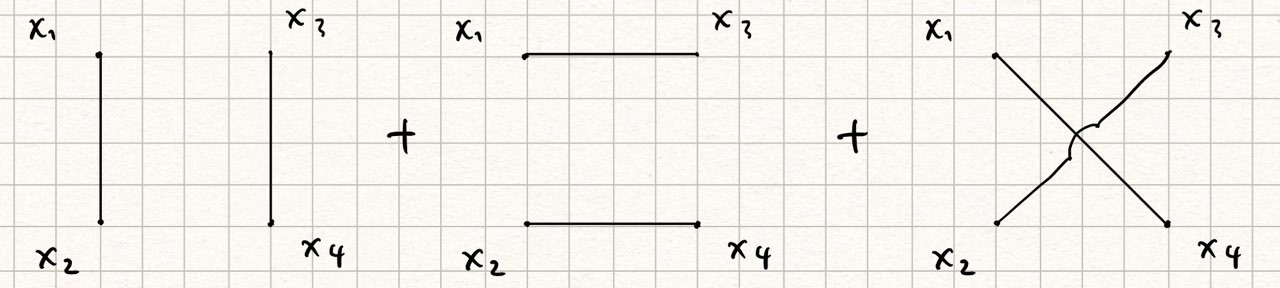
\includegraphics[width=0.7\linewidth]{4-3-feynman.jpg}
	\caption{Feynman diagrams}
	\label{fig:4-3-feynman}
\end{figure}
